%% use this to transform the beamer in an article
%\documentclass[12pt]{article}
%\usepackage[noxcolor]{beamerarticle}


\documentclass[aspectratio=169]{beamer}
\usefonttheme{serif}
%\documentclass[serif]{beamer}  % for 4:3 ratio
\usepackage[T1]{fontenc} 
\usepackage[spanish]{babel}
\usepackage{hyperref}
\usepackage{latexsym,amsmath,xcolor,multicol,booktabs,calligra}
\usepackage{graphicx,pstricks,listings,stackengine}
\usepackage{lipsum}
\usepackage{hyperref}

\author{Joaquín Mateos Barroso}
\title{Máquina Enigma y Máquina de Turing}
\subtitle{Cómo el análisis combinatorio salvó miles de vidas\\  
y Alan Turing creó el marco teórico para la codificación en ordenador}
\institute{
   i22mabaj@uco.es  \\  
    Códigos y Criptografía \\  
    Profesor: Jónatan Herrera Fernández  \\ 
    4$^o$ Ingeniería Informática
    \\  Universidad de Córdoba  \\  
}
\date{\small \today}
\usepackage{HKUSTstyle}

% defs
\def\cmd#1{\texttt{\color{red}\footnotesize $\backslash$#1}}
\def\env#1{\texttt{\color{blue}\footnotesize #1}}
% set colors
\definecolor{hkustyellow}{RGB}{167, 131, 55}
\definecolor{hkustblue}{RGB}{0, 56, 116}
\definecolor{hkustred}{RGB}{209, 51, 59}


\lstset{
    basicstyle=\ttfamily\small,
    keywordstyle=\bfseries\color{deepblue},
    emphstyle=\ttfamily\color{deepred},    % Custom highlighting style
    stringstyle=\color{deepgreen},
    numbers=left,
    numberstyle=\small\color{halfgray},
    rulesepcolor=\color{red!20!green!20!blue!20},
    frame=shadowbox,
}

%- --- --- --- --- --- --- --- --- --- --- --- --- --- --- --- 
\begin{document}

\begin{frame}
    \titlepage
    \vspace*{-0.6cm}
    \begin{figure}[htpb]
        \begin{center}
            
\includegraphics[keepaspectratio, scale=0.05]{pic/UCO-logo.png}
        \end{center}
    \end{figure}
\end{frame}


\begin{frame}    
\tableofcontents[sectionstyle=show,
subsectionstyle=show/shaded/hide,
subsubsectionstyle=show/shaded/hide]
\end{frame}

% Introduction --- --- --- --- --- --- --- --- --- --- --- --- 

\section{Contexto criptográfico}
\begin{frame}{Cifrado César}
	\begin{block}{Funcionamiento}
		Dado un número cualquiera $n\in \{0, ..., 25\}$, el cifrado César de desplazamiento $n$ de una letra, codificada en $\mathbb Z_{26}$, se define como
  $$E_n(x) := (x+n)\mod 26$$
	\end{block}
        
	\begin{block}{Vulnerabilidades. ?`Por qué es fácilmente descifrable?}
		\begin{itemize}
			 \pause \item Únicamente hay 26 formas de encriptación.
			 El análisis de frecuencias es muy sencillo.
                 \pause \item Hay que mandar la clave $n$.
		\end{itemize}
            Distintos algoritmos resolvieron parcialmente estos problemas, pero la Máquina Engima tiene mecanismos para resolver los 2 primeros muy efectivamente, y el último parcialmente.
	\end{block}
\end{frame}

\begin{frame}{Cifrado de Vigenère}
	\begin{block}{Funcionamiento}
		Dada una tupla de números $(c_1, ..., c_r)$, siendo $c_i\in \{0, ..., 25\}$, el cifrado de Vigenère de clave $(c_1, ..., c_r)$ de una frase $x_1x_2\cdots x_n$, codificada en $\mathbb Z_{26}$, se define como
  $$E_n(x_1x_2\cdots x_n) := (x_1+c_1), \cdots, (x_{r+1}+c_1), \cdots, (x_n + c_{n \% r+1}) \mod 26$$
	\end{block}
 
	\begin{block}{Ventajas y vulnerabilidades}
		\begin{itemize}
			 \pause \item Ya hay $26^r$ formas de encriptación, suficientes para la época.
			 \pause \item Buscando series de grupos de letras que se repitan periódicamente, se puede deducir el número de letras de la clave, y a partir de ahí hacer $r$ análisis de frecuencias.
                 \pause \item Hay que mandar la clave $(c_1, ..., c_r)$.
		\end{itemize}
	\end{block}


\end{frame}

\begin{frame}{?`Qué buscaban en una encriptación?}
    Se desarrollaron diversos métodos, pero si el ``enemigo`` capturaba a un soldado aliado, podía sacarle la información del encriptado.\pause \\  
    Tenían 3 objetivos principales:
	\begin{enumerate}
	     \pause \item Una gran cantidad de formas de encriptación.
             \pause \item Evitar el análisis de frecuencias.
             \pause \item Aunque se le informe al enemigo de la forma y clave de encriptación, podemos seguir comunicándonos con otros soldados.
	\end{enumerate}
    Enigma logró los 3 objetivos.

\end{frame}

% Literature Review --- --- --- --- --- --- --- --- --- --- --- 
\section{La Máquina Enigma}
\begin{frame}{La Máquina Enigma}
\centering
    Los alemanes crearon una máquina con varios rotores (en este caso 3) que se colocaban y giraban en función de sus necesidades.
    \begin{figure}

           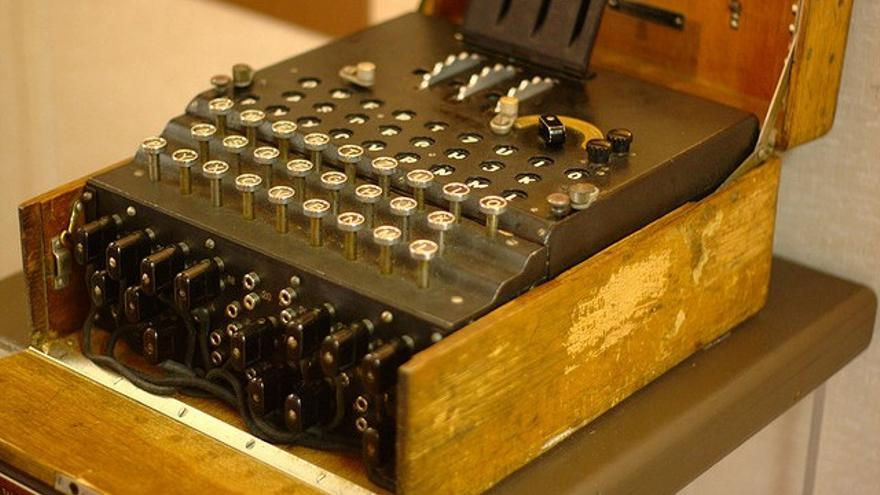
\includegraphics[width=0.5\linewidth]{pic/Máquina Enigma.png}
           \caption{Imagen de una Máquina Enigma real.}
           \label{fig:maquina-enigma}
    \end{figure}   

\end{frame}

\begin{frame}{La Máquina Engima}

\begin{figure}
    \centering
    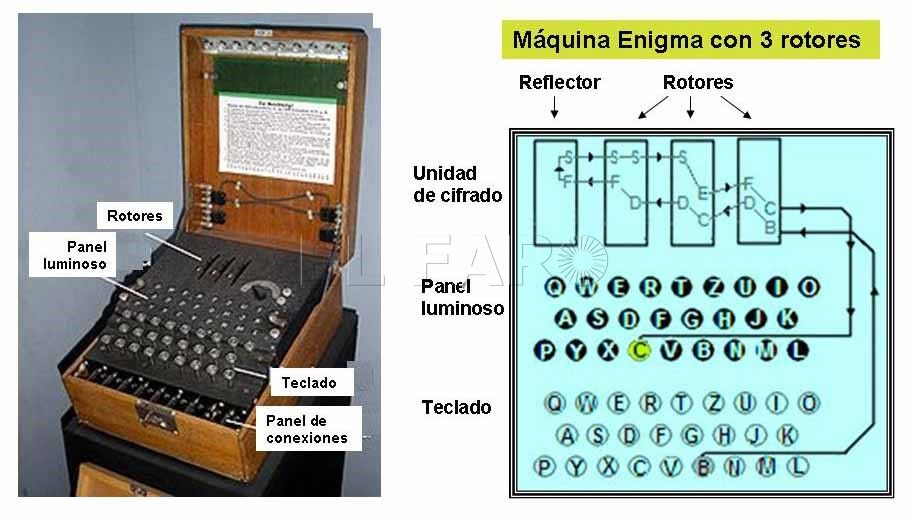
\includegraphics[width=0.75\linewidth]{Máquina Engima 2.png}
    \caption{Representación interna de la Máquina Enigma.}
    \label{fig:enter-label}
\end{figure}

\end{frame}

\begin{frame}{Vídeo demostrativo del funcionamiento de la Máquina Enigma}

    \begin{center}
        \href{https://drive.google.com/file/d/1BkQ4bM_GbFqefPEDQ3nXsJCX1MAV7sGi/view?usp=sharing}{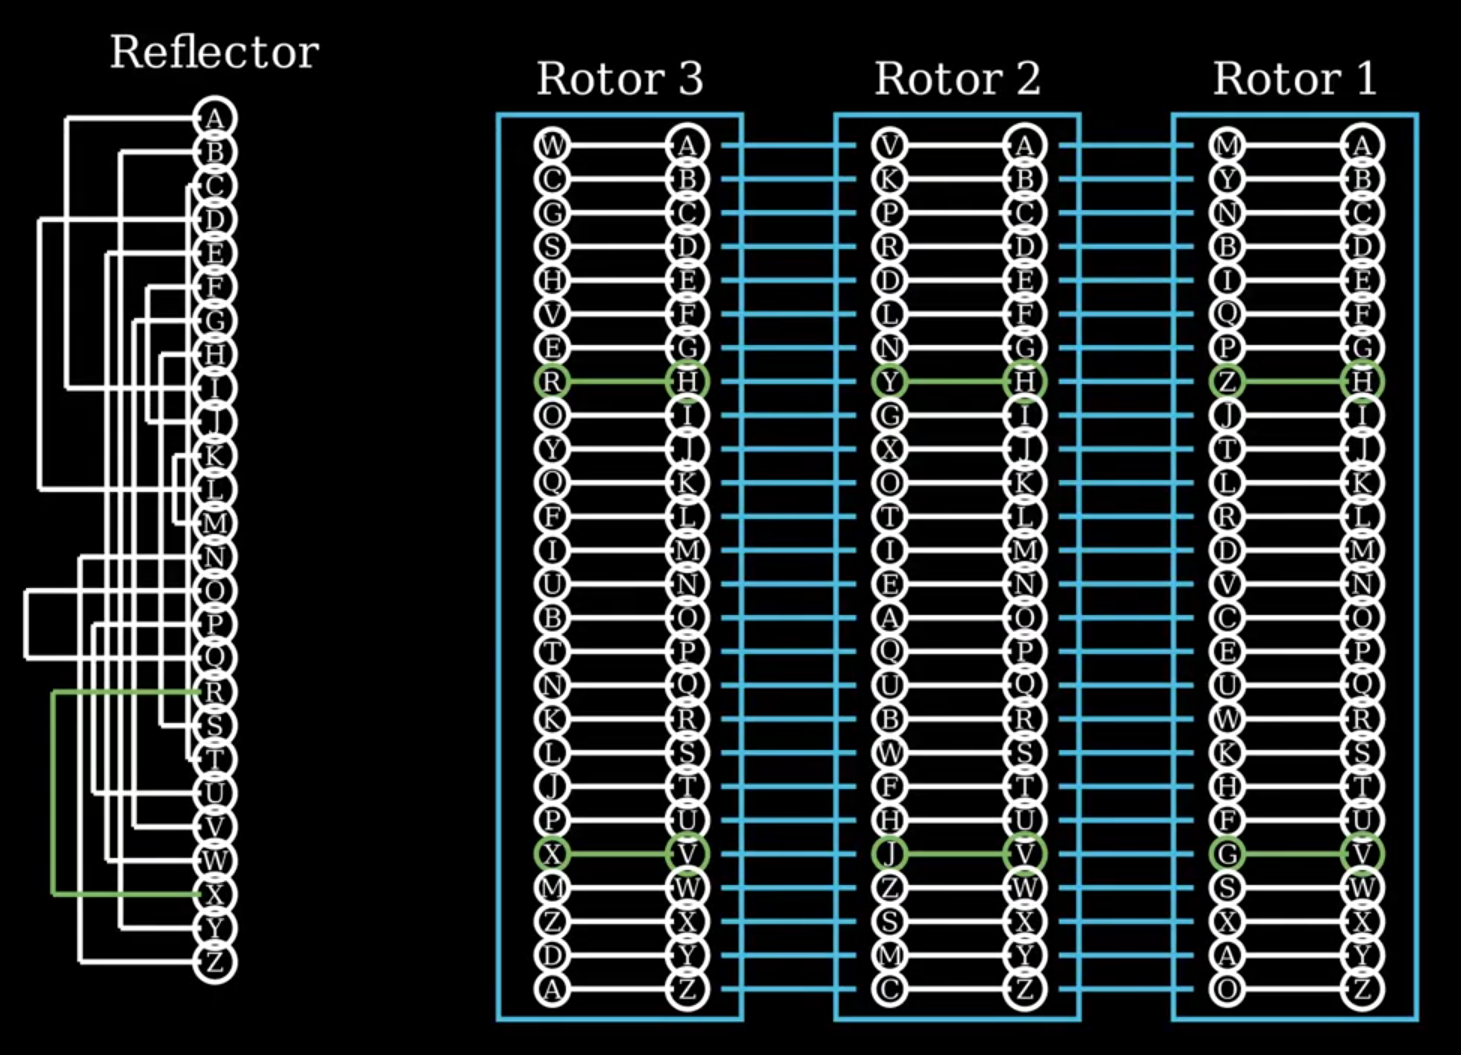
\includegraphics[width=0.7\textwidth,height=0.7\textheight,keepaspectratio]{pic/video-placeholder.png}}
    \end{center}
\end{frame}

\begin{frame}{Modelización matemática de Enigma}
    \begin{block}{Características matemáticas de sus componentes}
        \begin{enumerate}
         \pause \item 
        Cada rotor internamente realiza siempre la misma permutación. Llamemos a estas permutaciones $\sigma_1, \sigma_2, \sigma_3:\mathbb Z_{26} \rightarrow Z_{26}$, en orden de derecha a izquierda.
         \pause \item
        Dada una configuración inicial, en una iteración $k$, para pasar de un rotor, $i$, a otro, $i+1$, se está realizando una permutación $p^{(k)}_{i+1\leftarrow i}:\mathbb Z_{26} \rightarrow \mathbb Z_{26}$.
         \pause \item 
        Al volver, esta permutación se invierte; $p^{(k)}_{i+1\rightarrow i} = (p^{(k)}_{i+1\leftarrow i})^{-1}$.
         \pause \item        
        Por último, al llegar al reflejo final, se realiza una permutación $r:\mathbb Z_{26} \rightarrow \mathbb Z_{26}$ con la importante propiedad de que, al ser un reflejo, es involutivo, es decir, $r^{-1} = r$. Esta propiedad es muy importante para el descifrado sencillo de mensajes.
        
        \end{enumerate}
    \end{block}
\end{frame}

\begin{frame}{Modelización matemática de Enigma}
    \begin{block}{Características matemáticas de sus componentes}
Así, en la iteración $k$, si definimos 
$$pasoAIzquierda(x) := \sigma_3 \circ p_{3\leftarrow 2}\circ \sigma_2  \circ p_{2\leftarrow 1}\circ \sigma_1(x)$$
$$ pasoADerecha(x) := \sigma_1^{-1} \circ p_{2\rightarrow 1}\circ \sigma_2^{-1}  \circ p_{3\rightarrow 2}\circ \sigma_3^{-1}(x) $$
entonces la aplicación de la Máquina a una letra $x\in \mathbb Z_{26}$ sería
$$E_k(x) =  pasoADerecha \circ r \circ pasoAIzquierda \;(x)$$
    \end{block}
\end{frame}

\begin{frame}{Modelización matemática de Enigma}
    \begin{block}{Involución del encriptado de la Máquina Enigma}
        \textbf{Proposición.} El encriptado Enigma para un mismo paso $k$ es involutivo, i.e., $E_k^{-1} = E_k$.
    \end{block}
    
    \textbf{Demostración.} (Posiblemente sería mejor hacerla en pizarra, explicando los pasos)\pause \\  
    $$E_k^{-1} = pasoAIzquierda^{-1} \circ r^{-1} \circ pasoADerecha^{-1} =$$
    $$= \big(\sigma_1^{-1} \circ p_{2\leftarrow 1}^{-1}\circ \sigma_2^{-1}  \circ p_{3\leftarrow 2}^{-1}\circ \sigma_3^{-1}\big) \circ r \circ \big(  \sigma_3 \circ p_{3\rightarrow 2}^{-1}\circ \sigma_2  \circ p_{2\rightarrow 1}^{-1}\circ \sigma_1\big)=$$
    $$ \big( \sigma_1^{-1} \circ p_{2\rightarrow 1}\circ \sigma_2^{-1}  \circ p_{3\rightarrow 2}\circ \sigma_3^{-1}\big) \circ r \circ \big(\sigma_3 \circ p_{3\leftarrow 2}\circ \sigma_2  \circ p_{2\leftarrow 1}\circ \sigma_1\big) =$$
    $$= pasoADerecha \circ r \circ pasoAIzquierda = E_k$$
\end{frame}

\begin{frame}{Modo de empleo alemán}
Sin embargo, los alemanes no podían elegir una configuración y quedarse con ella, pues entonces cualquiera que obtuviera una máquina podría descifrar los mensajes.\pause \\  
Lo bueno es que para una máquina, hay $\binom{3}{2}$ ordenes de rotores, y 26 posiciones por rotor, luego hay $6\cdot 26^3 = 105, 456$ configuraciones distintas.
\begin{block}{Modo de empleo}
\begin{enumerate}
     \pause \item Al principio de cada mes, se mandaba una libreta con una configuración diaria.
     \pause \item El emisario coloca la configuración que toque, y manda 2 veces una terna de letras elegidas, e.g., STGSTG. A continuación inicializa cada rotor con la letra elegida.
     \pause \item El receptor lee las 6 primeras letras, coloca los rotores como corresponda, y lee el resto del mensaje.
\end{enumerate}
\end{block}
\end{frame}


\begin{frame}{Modo de empleo alemán}
\begin{block}{Ventajas}
\begin{itemize}
     \pause \item Inutiliza el análisis de frecuencias.
     \pause \item Hace falta la libreta mensual para descifrar mensajes.
     \pause \item Aún si se intercepta un trozo de mensaje y se tiene la libreta, hace falta el inicio del mensaje para entenderlo.
     \pause \item Una configuración distinta cada día, y en cada mensaje.
\end{itemize}
\end{block}
\begin{block}{Inconvenientes}
\begin{itemize} 
     \pause \item No es trivial mandar mensualmente la libreta.
     \pause \item Mandar 2 veces las mismas letras trae problemas... Lo veremos a continuación.
     \pause \item Alan Turing no era alemán.
     \pause \item Hay una película que se llama ``Descifrando Enigma``, así que algo pasaría.
\end{itemize}
\end{block}


\end{frame}



% Methods --- --- --- --- --- --- --- --- --- --- --- 
\section{Descifrando Enigma}
\begin{frame}{Problema a resolver}
Cuando empezó la guerra, los alemanes, viendo que los polacos estaban realizando progresos, añadieron un proceso de cableado previo, en el que 6 letras del alfabeto original se cambiaban por otras 6 para ser introducidas en el primer rotor.\pause \\  
De esta forma, había $\binom{26}{12}$ formas de elegir las letras, y $\frac{1}{2^6} \cdot \binom{12}{6} \cdot 6!$ formas de elegir la forma en la que conectamos estas 12 letras.\pause \\  

En total, hay 
$$105,456 \cdot \binom{26}{12} \cdot \frac{1}{2^6} \cdot \binom{12}{6} \cdot 6! \sim 10^{16}$$
configuraciones distintas de la máquina. Creando así un sistema inviable de estudiar por ningún método ni remotamente exhaustivo.

\end{frame}

\begin{frame}{Solución de Marian Rejewski}
\begin{columns}
    \begin{column}{0.5\textwidth}
        Los polacos consiguieron interceptar algunas máquinas Enigma, y, gracias a un equipo de grandes matemáticos que había allí en la época, consiguieron grandes resultados. En particular, uno de ellos, \textit{Marian Rejewski}, desarrolló un método que permitió la desencriptación de los mensajes alemanes.

    \end{column}
    \begin{column}{0.5\textwidth}
        \begin{figure}
            \centering
            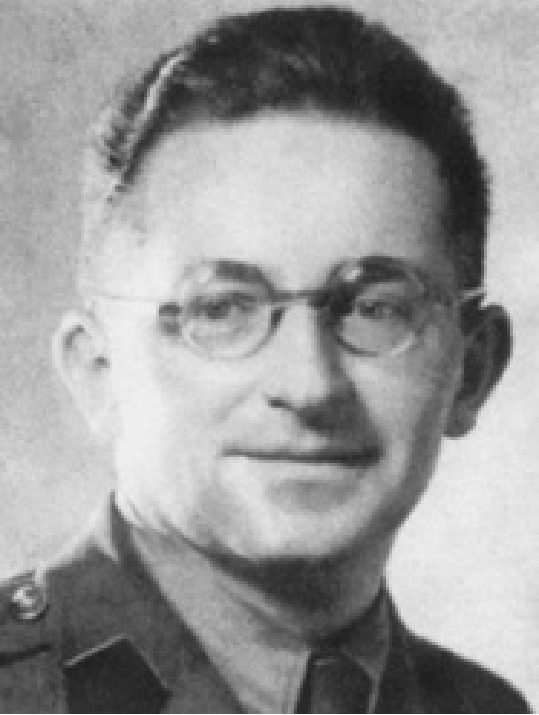
\includegraphics[width=0.5\linewidth]{pic/Rejewski.png}
            \caption{Marian Rejewski.}
        \end{figure}
    \end{column}
\end{columns}
\end{frame}

\begin{frame}{Solución de Marian Rejewski}
Rejewski se dio cuenta de que las repeticiones de caracteres entre las 6 primeras letras daban mucha información.\pause \\  
Primero ordenaba varios mensajes de la siguiente forma:
\begin{figure}
    \centering
    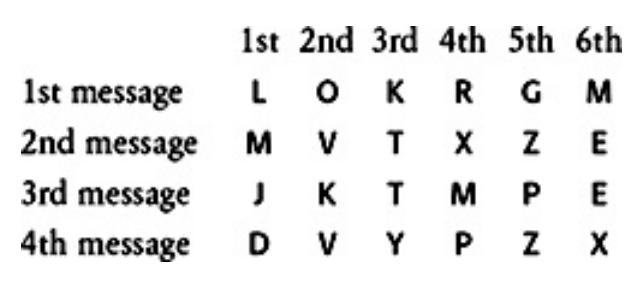
\includegraphics[width=0.5\linewidth]{pic/ordenacion1.png}
\end{figure}

\begin{figure}
    \centering
    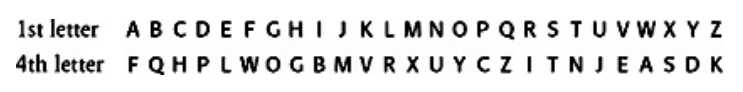
\includegraphics[width=0.75\linewidth]{pic/ordenacion2.png}
\end{figure}
    
\end{frame}

\begin{frame}{Solución de Marian Rejewski}
Con esta información, y la de los pares de letras (2, 5), (3, 6), que correspondían, originalmente, a la misma letra, se dio cuenta de que se cumplía una propiedad interesante de las \textit{cadenas de Rejewski} de permutaciones generadas:

\begin{figure}
    \centering
    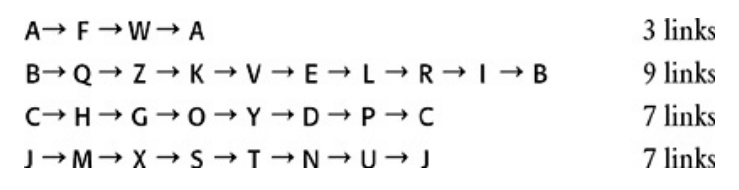
\includegraphics[width=0.6\linewidth]{ordenacion3.png}
\end{figure}
Esta propiedad consiste en que la longitud de estas cadenas era constante sin importar el orden del cableado de 6 pares de letras inicial.\pause \\  
Así se redujo la cantidad de configuraciones a explorar al mismo que sin cableado; $105,456$ configuraciones. Pero Rejewski tenía un truco más.
\end{frame}

\begin{frame}{Solución de Marian Rejewski}
Primero encargó a su equipo que recopilara las cadenas generadas por las $105,456$ posibles configuraciones.\pause \\  
Tras un año, las obtuvieron todas, y, viendo el invariante anterior, las catalogaron de acuerdo a esta información de la siguiente forma:
\begin{figure}
    \centering
    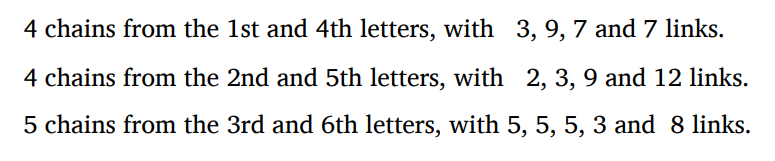
\includegraphics[width=0.5\linewidth]{pic/ordenacion4.png}
\end{figure}
Esto es un invariante de la cadena, y además cada cadena tiene una única forma de entre estas.\pause \\  
Gracias a todo esto, Rejewski consiguió descifrar Enigma.

\end{frame}

\begin{frame}{Solución de Marian Rejewski}
\begin{block}{Primera solución de Enigma}
    \begin{enumerate}
         \pause \item Rejewski recopilaba mensajes del día hasta obtener las cadenas correspondientes a las primeras letras.
         \pause \item A partir de este invariante, descubría la estructura de rotores que tenían las máquinas ese día en particular.
         \pause \item Con los rotores en posición, el juego era trivial, pues estaban todas las letras, menos 12, colocadas correctamente, luego se buscaban frases como \textit{alliveinbelrin}, que se suponía que significaba \textit{arrive in Berlin}, por lo que se sustituía la \textit{r} por la \textit{l} en el cableado, y se proseguía hasta terminar.
    \end{enumerate}
\end{block}

\end{frame}

\begin{frame}{Alan Turing}

\begin{columns}
    \begin{column}{0.5\textwidth}
Alan Turing fue un matemático británico pionero en la computación teórica y la inteligencia artificial. Su trabajo en la Máquina de Turing sentó las bases de la ciencia de la computación moderna. Sus contribuciones a la lógica matemática y la teoría de la computabilidad son fundamentales en la informática actual.
        
    \end{column}
    \begin{column}{0.5\textwidth}
        \begin{figure}
            \centering
    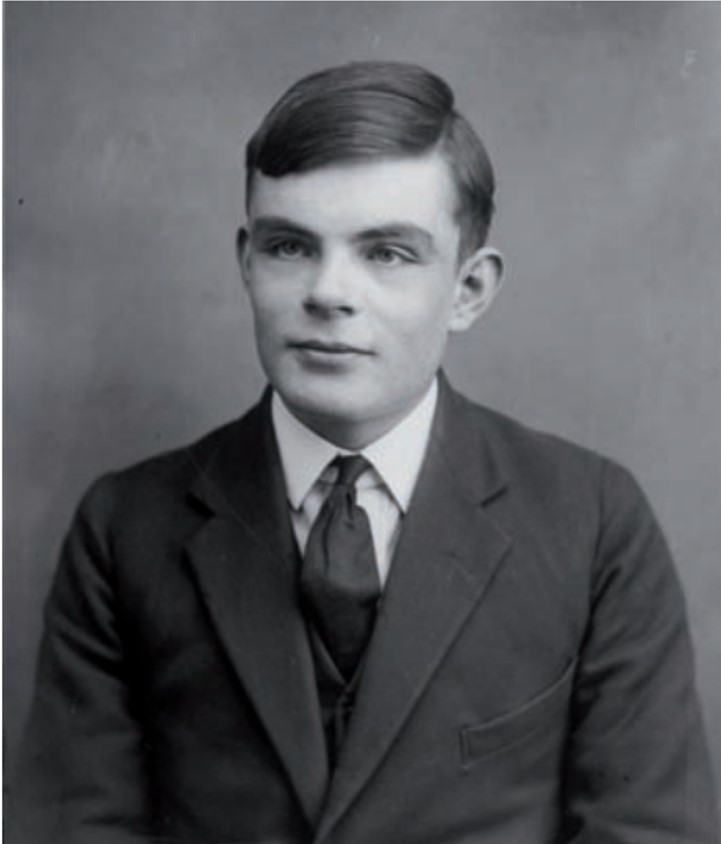
\includegraphics[width=0.65\linewidth]{pic/Alan Turing.png}
            \caption{Alan Turing.}
        \end{figure}
    \end{column}
\end{columns}
\end{frame}

\begin{frame}{Bletchley Park}

\begin{columns}
    \begin{column}{0.5\textwidth}
    Los británicos construyeron en Bletchley Park una instalación militar en la que reunieron a los mejores científicos, matemáticos, ajedrecistas y resolvedores de crucigramas del país para resolver Enigma.\\
    Entre ellos estaba nuestro protagonista; Alan Turing.

    \end{column}
    \begin{column}{0.5\textwidth}
        \begin{figure}
            \centering
    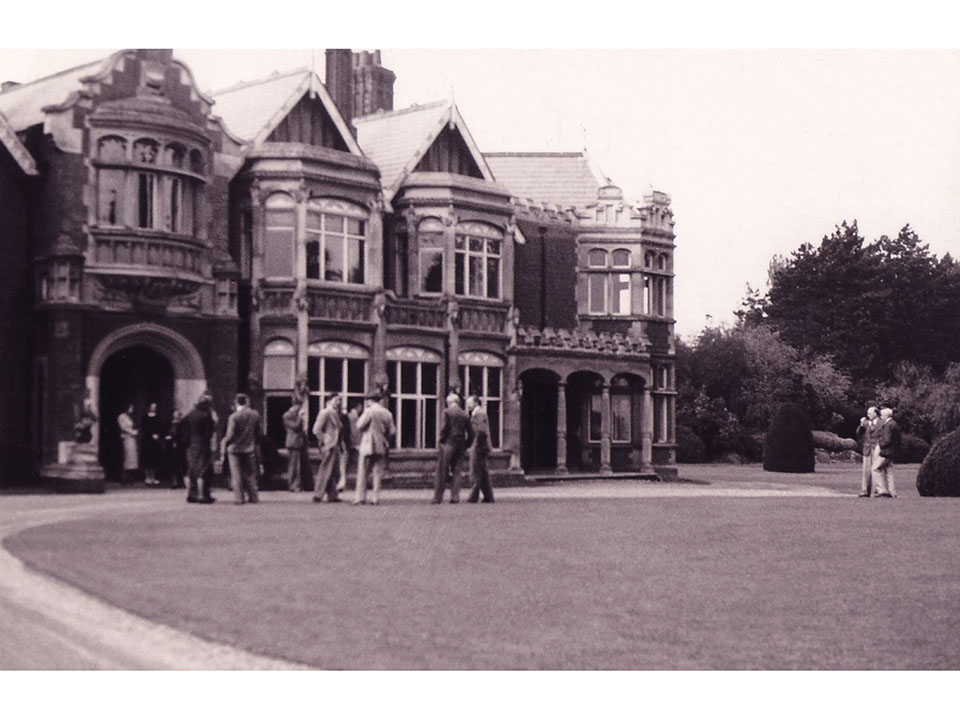
\includegraphics[width=0.65\linewidth]{pic/bletchley-park.png}
            \caption{Bletchley Park.}
        \end{figure}
    \end{column}
\end{columns}
\end{frame}


\begin{frame}{Problema al que se enfrentaron desde Bletchley Park}
Los alemanes habían sofisticado un poco la máquina al ver los esfuerzos de Rejewski.
\begin{itemize}
    \item Aunque seguían usando 3 discos, ahora tenían 5 con los que intercambiar. Así había $\binom{5}{2}\cdot 3! = 60$ posiciones de discos.
    \item Juntando esto con las rotaciones, se llegó a $60 \cdot 26^3 = 1, 054, 560$ configuraciones de rotores.
    \item Añadieron más intercambios iniciales de letras por cableado, llegando en total a unas $1'59\cdot 10^{20}$ configuraciones.
\end{itemize}
Gracias a estos cambios inutilizaron el algoritmo de Rejewski.
\end{frame}




\begin{frame}{Solución de Alan Turing}
Alan Turing, siguiendo la idea de las \textit{cadenas de Rejewski}, definió los \textbf{bucles de Turing} como aquellos conjuntos de letras tales que Enigma, en una configuración en particular, transformaba la primera letra en la segunda, la segunda en la tercera, etc., consecutivamente.
\pause
\begin{figure}
	\centering
	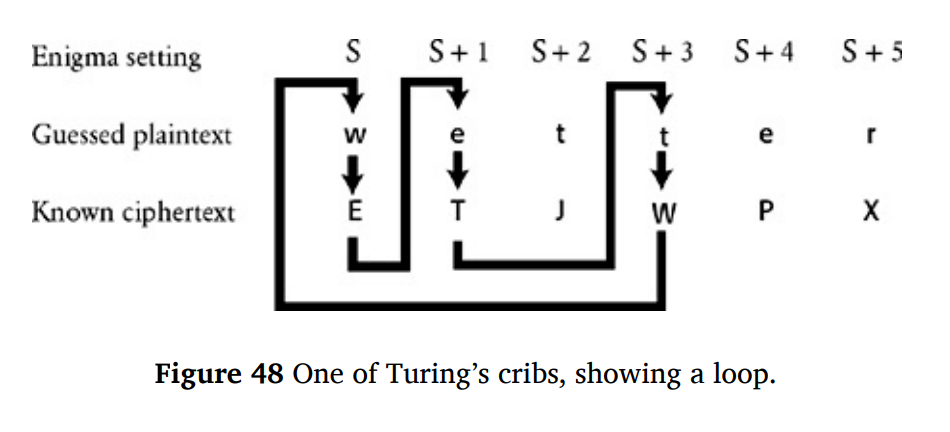
\includegraphics[width=0.6\linewidth]{pic/bucleDeTuring}
\end{figure}
\end{frame}

\begin{frame}{Solución de Alan Turing}
	De esta forma, cada día Turing creaba los siguientes resúmenes:
	\pause
	\begin{figure}
		\centering
		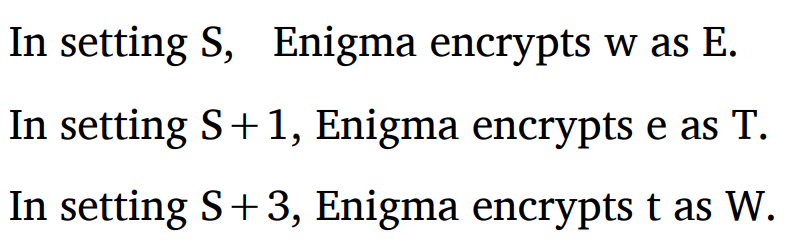
\includegraphics[width=0.4\linewidth]{pic/bucleDeTuring1}
	\end{figure}
	Estos resúmenes no identificaban inequívocamente a una configuración, pero eran una gran criba.\\
	\pause
	El problema aún así es que era inviable aplicar esta criba sobre las $1'59\cdot 10^{20}$ configuraciones.\\
	Aquí llegó otra idea magnífica de Turing, la cual cambió el juego.
\end{frame}

\begin{frame}{Bombe}
	\begin{columns}
		\begin{column}{0.5\linewidth}
			Turing imaginó la terna de máquinas que tenemos a la derecha. Cada máquina comprueba uno de los 3 elementos del \textit{bucle} que sabemos que se cumple, y, en caso de que las 3 devuelvan la letra correcta, se enciende la bombilla.\\

			Para resolver el problema del cableado o \textit{plugboard}, Turing, en lugar de trabajar a nivel teórico con las letras dadas, trabajaba en abstracto con $L_1, L_2, L_3$.
		\end{column}
		\begin{column}{0.35\linewidth}
			
			\begin{figure}
				\centering
				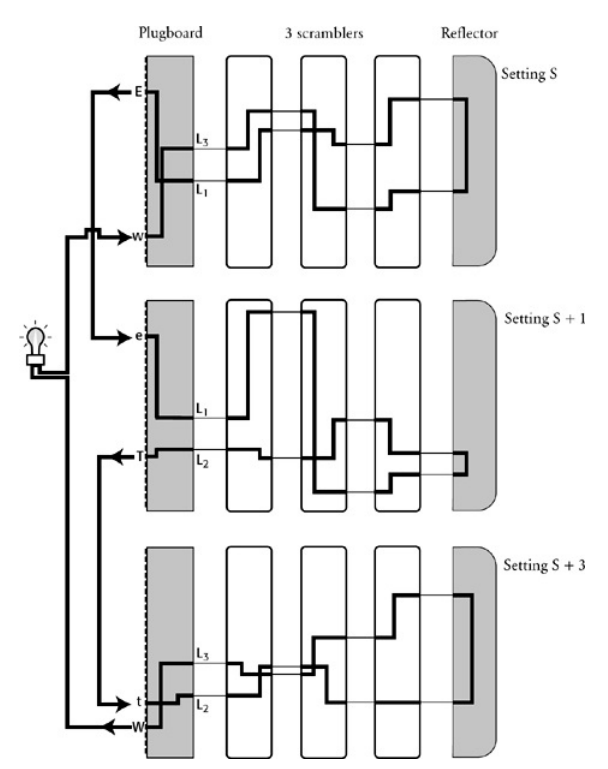
\includegraphics[width=0.9\linewidth]{pic/bucleDeTuring2}
				\caption{Modelización teórica de \textit{Bombe}.}
			\end{figure}
		\end{column}
	\end{columns}
\end{frame}


\begin{frame}{Solución de Turing}
	\begin{block}{Cómo Turing descifró Enigma; \textit{Victory}}
		Apodaron Victory a la primera máquina física que implementó esta idea teórica.
		\begin{enumerate}
			\item Cada día, los criptógrafos buscaban \textit{bucles de Turing}. \pause
			\item A continuación, se introducen los bucles a \textit{Victory}, que calculaba la estructura interna de rotores de la máquina. Si se comprobaba una de las $17,576$ orientaciones por segundo (en realidad se era más rápido), se había encontrado el sistema en, máximo, 5 horas. \pause
			\item Una vez se tiene la estructura interna, al igual que con Rejewski, se prueban cableados hasta encontrar el correcto. \pause
		\end{enumerate}
	\end{block} \pause
	Con este sistema se consiguió descifrar Enigma, y se salvaron miles de vidas.
\end{frame}

\begin{frame}
	
	\begin{columns}
		\begin{column}{0.6\linewidth}
			A lo largo de la guerra se siguieron produciendo pequeños cambios en el sistema alemán, cuando iban dándose cuenta de que los descubrían.\\
			Sin embargo, gracias a las brillantes mentes en Bletchley Park, todas se descifraron.\\
			Un caso importante es el de \textit{Tommy Flowers}, ingeniero electrónico que, basándose en muchas de las ideas teóricas desarrolladas allí, creó \textbf{Collosus}, el que por muchos es considerado el primer computador digital.\\
			Sin embargo, debido a la clasificación de esta información por el gobierno británico, nos queda una pequeña porción de lo que se desarrolló allí, y pocos investigadores consiguieron reconocimiento.
		\end{column}
	
		\begin{column}{0.4\linewidth}
			\begin{figure}
			\centering
			\includegraphics[width=0.7\linewidth]{"pic/Tommy Flowers"}
			\caption{Tommy Flowers}
			\end{figure}
		\end{column}
	\end{columns}
	
\end{frame}

% Results --- --- --- --- --- --- --- --- --- --- --- 
\section{Codificación teórica mediante la Máquina de Turing}

% --- Thank you slide ---
\begin{frame}
\begin{center}
{ Muchas gracias por escuchar !}
\vspace{1cm}

Joaquín Mateos Barroso \\  [1em]
i22mabaj@uco.es 
\end{center}
\end{frame}

\end{document}